\chapter{Resultados}

\section{Introducción}
%
Los resultados obtenidos en cada uno de los pasos de este trabajo se detallan en
este capítulo, comenzando por el motor obtenido en la primer iteración de
optimización con el algoritmo genético, luego se presenta el modelo de CAD
generado para la segunda etapa de simulación.

Luego se muestran los resultados de las flujometrías realizadas con la geometría
obtenida, incluyendo las mallas obtenidas para algunos casos seleccionados y el
resultado detallado de algunas de las flujometrías, finalizando con el mapa de
coeficientes de descarga obtenido, tanto para el puerto de admisión como para el
puerto de escape.

Por último se presentan los resultados de la segunda ronda de optimización con
el algoritmo genético, en la que se utilizó el mapa de coeficientes de descarga
obtenido en el paso previo.
%
En esta sección se muestra además el modelo de CAD generado para esta geometría.

\section{Primer Iteración}
%
La primer optimización se realizó partiendo de una población al azar, con los
coeficientes de descarga constantes de 0.7 y 0.75 para el puerto de admisión y
escape respectivamente.
%
El algoritmo genético se ejecutó durante 100 generaciones con una población de
100 individuos, la función objetivo es la definida en la sección xxx con los
pesos indicados, los operadores y parámetros correspondientes indicados en la
tabla~\ref{tab:config_genetico}.

\begin{table}
  \centering
  \begin{tabular}{cc} \toprule
    Parámetro & Valor \\ \midrule
    RPMS & $(1000, 2000, 3000, 4000, 5000, 6000, 7000, 8000, 9000)$ \\
    Pesos de función objetivo & $(1, 1, 1, 6, 8, 9, 8, 7, 7)$ \\
    Cantidad de ciclos de ICESym & 2 \\
    Diámetro mínimo & 0.05 \\
    Diámetro máximo & 0.1 \\
    Longitud mínima de tubo & 0.5 \\
    Longitud máxima de tubo & 2 \\
    Ángulo mínimo & 0 \\
    Ángulo máximo & 90 \\
    Separación angular máxima & 70 \\
    Tamaño de población & 100 \\
    Tamaño de torneo & 10 \\
    $\mu$ & 0 \\
    $\sigma$ & 1 \\
    $\alpha$ & 0.5 \\
    Probabilidad de cruza & 0.9 \\
    Probabilidad de mutación & 0.5 \\
    Cantidad de generaciones & 20 \\
    Tamaño de \emph{SALÓN DE LA FAMA} & 1 \\ \bottomrule
    \end{tabular}
  \caption{Configuración utilizada.}\label{tab:config_genetico}
\end{table}


En la gráfica de evolución de la aptitud media y máxima de la población se ve
que se obtuvo rápidamente un individuo con un puntaje relativamente alto en la
generación X, un X porciento mayor a la media.
%
El resultado final tiene una aptitud XX mayor a la aptitud media de la
población, los parámetros que definen este candidato son los listados en la
tabla y se ilustran en la figura~\ref{fig:pop_ev_1}.
%
Este motor tiene un rendimiento volumétrico máximo de 0.8 para 1000 rpm y si
bien la función objetivo favorece curvas suaves, se ven dos picos de rendimiento
en la curva, siendo el segundo a 1100 rpm.

\begin{figure}
    \centering
    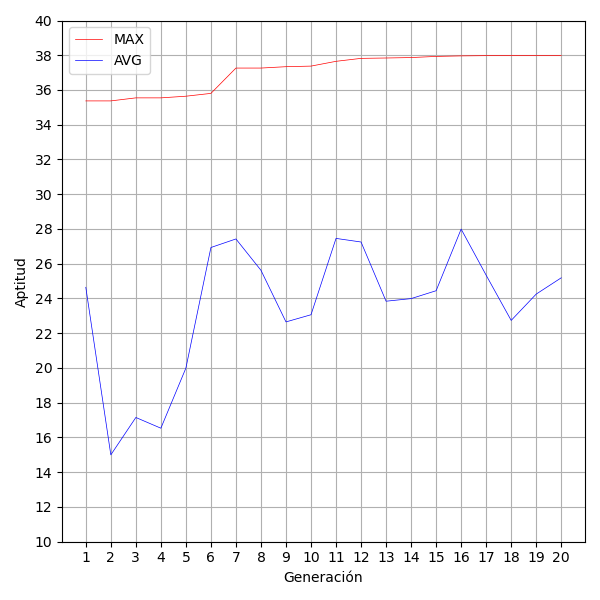
\includegraphics[width=.7\textwidth]{genetico/pop_evolution.png}
    \caption{Evolución de la primer optimización.}\label{fig:pop_ev_1}
\end{figure}

\begin{table}
  \centering
  \begin{tabular}{cc} \toprule
    Parámetro & Valor & Unidad \midrule
    DTA & 97.24 & mm\\
    DTE & 81.15 & mm\\
    LIT & 519.31 & mm\\
    LET & 976.66 & mm\\
    IIA & 1.12 & grado\\
    IFA & 70.15 & grado\\
    EIA & 85.14 & grado\\
    EFA & 11.13 & grado\\ \bottomrule
  \end{tabular}
  \caption{Mejor Candidato.}\label{tab:resultado_primer_it}
\end{table}


En la figura XXX se muestran las curvas de potencia y torque del motor, como es
de esperarse se ve que ambas copian la curva de rendimiento volumétrico, con una
potencia máxima de XXX HP a 1000 rpm y un torque máximo de xxxx N.m. a xxx rpm.

\subsection{Puerto de admisión}

Evaluando las curvas de presión para estas rpm se observa que durante la
apertura del puerto de escape hay una depresión de XXX Pa, para este punto el
coeficiente de descarga se estima en XXX y fluje un XX porciento de la masa
total que ingresa durante el período angular en que se encuentra abierto el
puerto.

El puerto de escape ocupa un período angular de $69^{\circ}$, inciando la
apertura en $1.12^{\circ}$ y cerrando a $70.15^{\circ}$ en relación al giro del
cigüeñal.

Se puede concluir que el puerto de admisión tiene sintonías en XXX, XXX, XXX rpm, siendo los diferenciales de presión mayores en xxx xxx xxx.

\subsection{Puerto de admisión}
%
El puerto de escape ocupa un período angular de $69^{\circ}$, inciando la
apertura en $1.12^{\circ}$ y cerrando a $70.15^{\circ}$ en relación al giro del cigüeñal.


\subsection{Modelo de CAD}
%
Los parámetros geométricos obtenidos se utilizaron para modelar los puertos,
tratando de generar una transición suave entre puerto y cámara de combustión
para favorecer el pasaje de gas.
%
Como se ve en la figura~\ref{fig:motor_cad}, se redondearon las aristas internas incluyendo las
paletas y las puntas del rotor, esto para favorecer el proceso de mallado
requerido en el paso siguiente a este ya que los bordes agudos son complejos de
adaptar a una malla construida con tetraedros, como lo es la malla resultante de
snappyHexMesh que se describió en el apartado xxx del capítulo xxx.

\begin{figure}
  \centering
    \begin{subfigure}{0.4\textwidth}
        \centering
        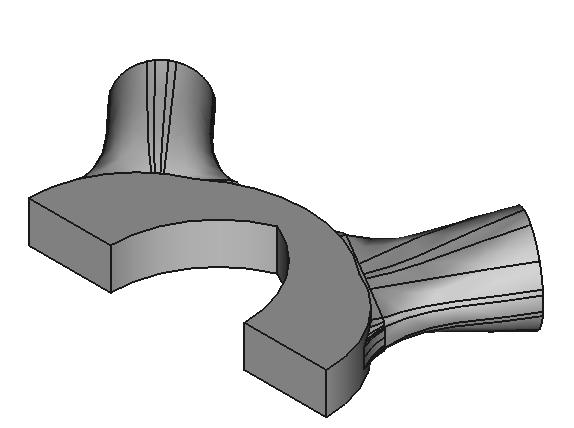
\includegraphics[width=\textwidth]{CAD/motor_cad1.png}
    \end{subfigure}
    \hfill
    \begin{subfigure}{0.4\textwidth}
        \centering
        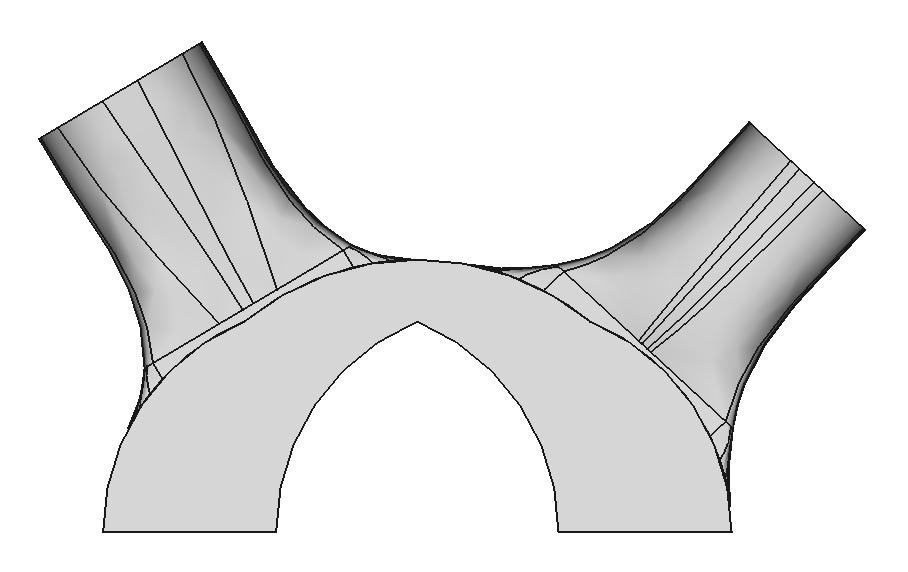
\includegraphics[width=\textwidth]{CAD/motor_cad2.png}
    \end{subfigure}
  \caption{CAD Primer Iteración}\label{fig:motor_cad1}
\end{figure}

La altura del puerto del lado de la cámara de combustión se mantuvo en dos
tercios del a altura de cámara.

\begin{figure}
  \centering
    \begin{subfigure}{0.8\textwidth}
        \centering
        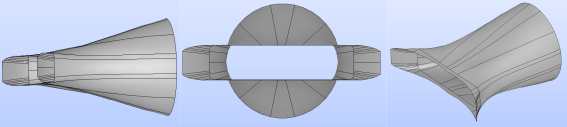
\includegraphics[width=\textwidth]{CAD/vistas_admision.png}
        \caption{Puerto de Admsisión.}
    \end{subfigure}
    \begin{subfigure}{0.8\textwidth}
        \centering
        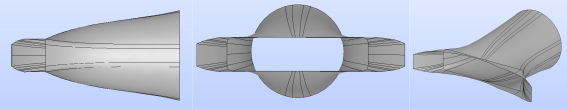
\includegraphics[width=\textwidth]{CAD/vistas_escape.png}
        \caption{Puerto de Escape.}
    \end{subfigure}
  \caption{CAD Primer iteración (vistas fuera de escala).}\label{fig:motor_cad2}
\end{figure}


\section{Flujometrías}

De los resultados de la primer otpimización se extrajo una curva de diferencia
de presión vs alzada para diferentes velocidades del motor para identificar los
puntos de mayor interés para realizar las fluometrías, tratando de obtener una
buena cobertura del rango de funcionamiento de cada puerto.

Inicialmente se propusieron un total de XXX flujometŕias, sin embargo algunas
combinaciones de $\l_{v}, \Delta P$ no se pudieron ejecutar hasta la
convergencia del flujo másico, por lo que se redujo la cantidad de flujometrías
final a xxx flujometrías, xxx para el puerto de admisión y xxx para el puerto de
escape, el par $(\l_{v}, \Delta P)$ se detalla en la figura XXX y tabla xxx.
%
Con estos datos se calculó el coeficiente de descarga para cada punto evaluado
obteniendo la base para generar el mapa de coeficientes de descarga que se
utilizará en el próximo paso de simulación, los valores de presión, alzada y
coeficiente de descarga obtenidos se listan en la tabla xxx.

Como se mencionó en el apartado~\ref{ch:mrcvc}, la modificaión realizada a
ICESym para funcionar con un mapa de $C_{D}$ dependiente de dos variables
requiere que los datos de entrada estén distribuidos en una grilla rectangular,
motivo por el cual a partir de estos valores se utilizó el método de
interpolación por IDW mencionado en el mismo apartado para generar una dicha
grilla de valores de $(l_{v}, \Delta P)$ con $C_{D}$ interpolado de los datos
conocidos, como se ve en las figuras~\ref{fig:mapa_cd_admision}
y~\ref{fig:mapa_cd_escape}.

\begin{figure}
    \centering
    \begin{subfigure}{0.4\textwidth}
        \centering
        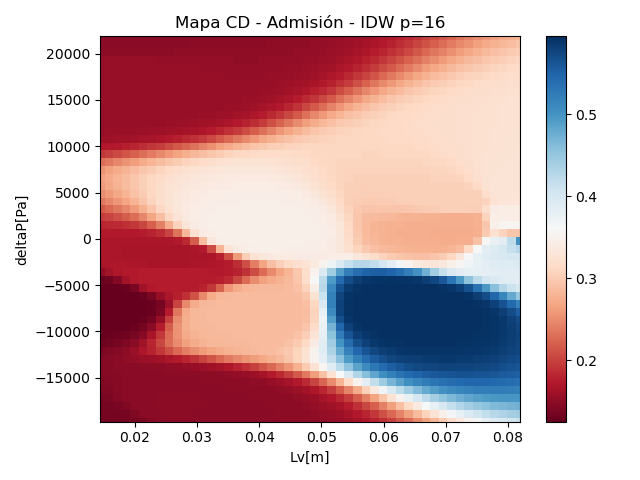
\includegraphics[width=\textwidth]{mapa_cd/idw16_mapa_adm.png}
        \caption{cambiar}
    \end{subfigure}
    \hfill
    \begin{subfigure}{0.4\textwidth}
        \centering
        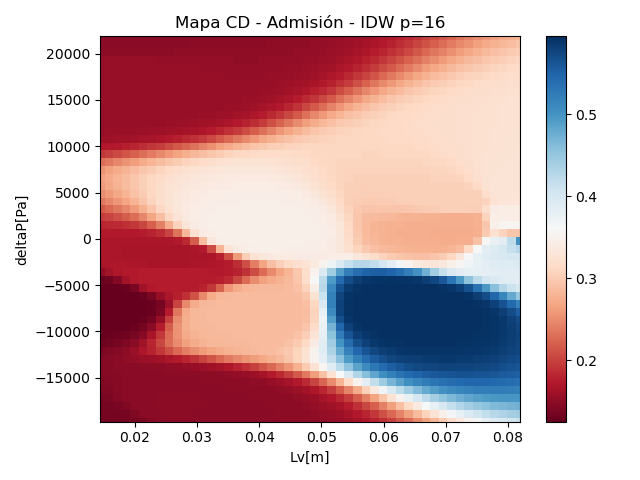
\includegraphics[width=\textwidth]{mapa_cd/idw16_mapa_adm.png}
        \caption{cambiar}
    \end{subfigure}
    \caption{cabmiar}\label{fig:mapa_cd_admision}
\end{figure}

\begin{figure}
    \centering
    \begin{subfigure}{0.4\textwidth}
        \centering
        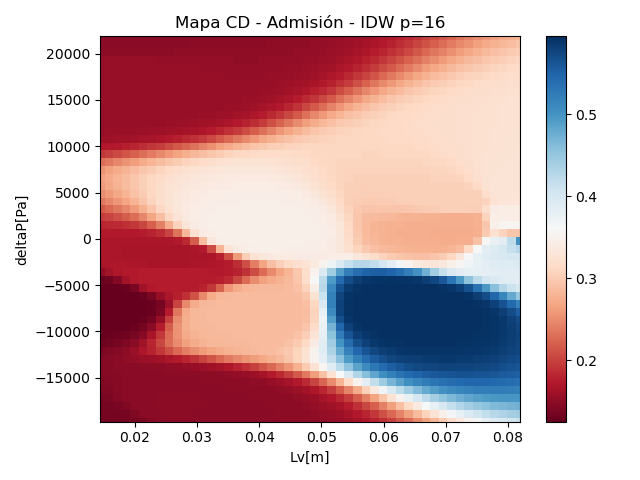
\includegraphics[width=\textwidth]{mapa_cd/idw16_mapa_adm.png}
        \caption{cambiar}
    \end{subfigure}
    \hfill
    \begin{subfigure}{0.4\textwidth}
        \centering
        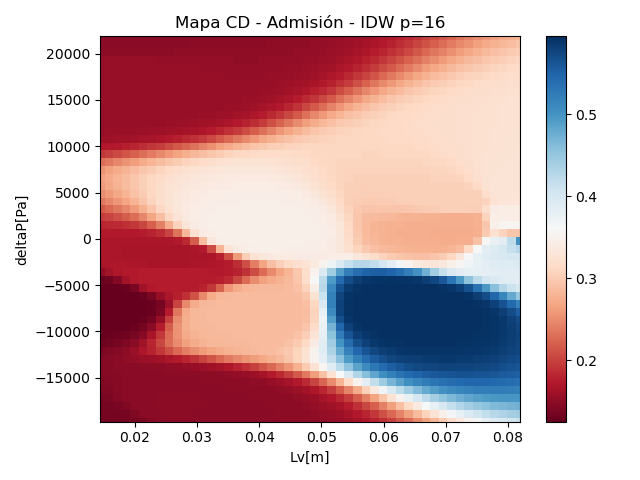
\includegraphics[width=\textwidth]{mapa_cd/idw16_mapa_adm.png}
        \caption{cambiar}
    \end{subfigure}
    \caption{cabmiar}\label{fig:mapa_cd_escape}
\end{figure}

En el mapa del puerto de admisioń se observa un máximo para para aperturas del
puerto mayores a 80mm, con $\Delta P$ de entre 1000 Pa a 15000 Pa.
%
El coefiente de descarga máximo es $C_{D}(100mm, 1500Pa) = 0.6$ y corresponde a
la flujometría $N^{\circ} X$, el flujo másico obtenido para este régimen es de
0.02 kg/s, con un a velocidad máxima de xxx m/s en la garganta.
%
El peor valor se es $C_{D}(100mm, 1500Pa) = 0.6$ y corresponde a aperturas
pequeñas del puerto, en la que debido a la reducida sección de pasaje de flujo
se tiene velocidades eleveadas, siendo la máxima de xxx m/s.
%
Para visualizar la diferencia entre uno y otro caso, se representan las líneas
de corriente para ambos casos en la figura \ref{fig:comparativa_lineas_corriente}.

\begin{figure}
    \centering
    \begin{subfigure}{0.4\textwidth}
        \centering
        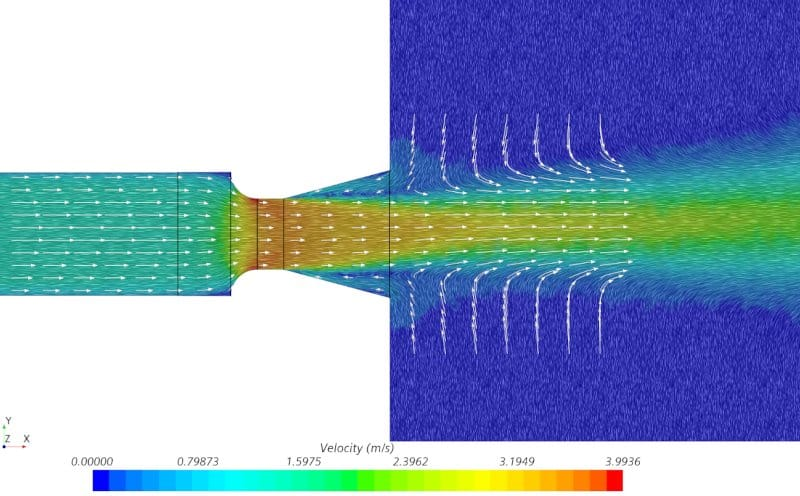
\includegraphics[width=\textwidth]{flujometrias/ejemplo_lineas_corriente.jpg}
        \caption{Valor máximo de $C_{D}$}
    \end{subfigure}
    \hfill
    \begin{subfigure}{0.4\textwidth}
        \centering
        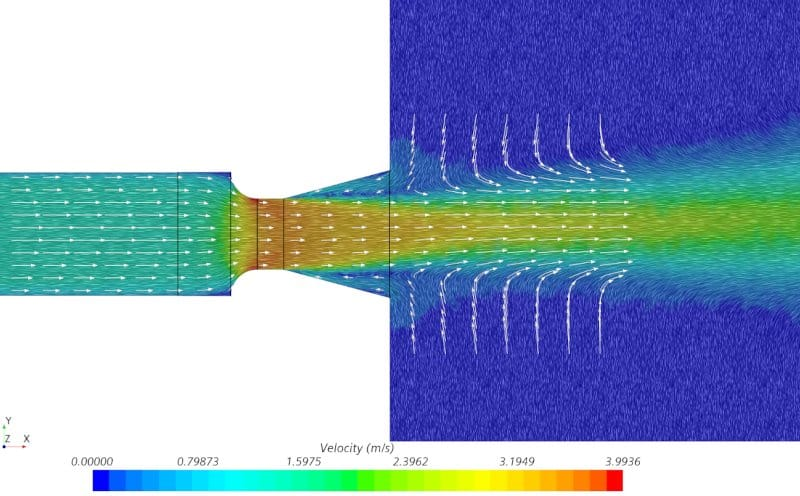
\includegraphics[width=\textwidth]{flujometrias/ejemplo_lineas_corriente.jpg}
        \caption{Valor mínimo de $C_{D}$}
    \end{subfigure}
    \caption{cabmiar}\label{fig:comparativa_lineas_corriente}
\end{figure}

Para el mapa del puerto de escape se observa un máximo para para aperturas del
puerto mayores a 80mm, con $\Delta P$ de entre 1000 Pa a 15000 Pa.
%
El coefiente de descarga máximo es $C_{D}(100mm, 1500Pa) = 0.6$ y corresponde a
la flujometría $N^{\circ} X$, el flujo másico obtenido para este régimen es de
0.02 kg/s, con un a velocidad máxima de 10m/s en la garganta, como se ve en la
figura \ref{fig:admision_10_2000.jpg}.

\begin{figure}
    \centering
    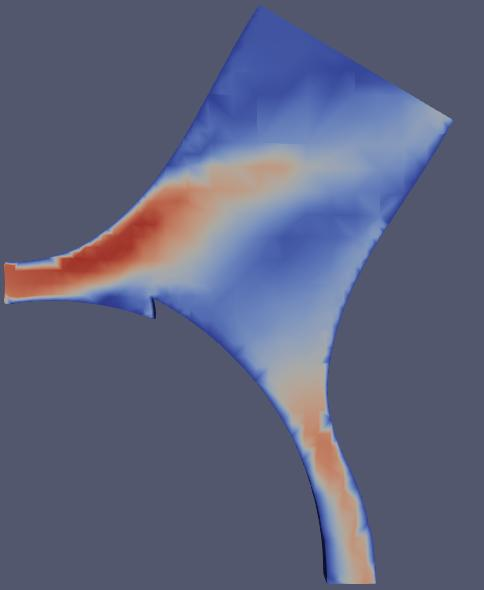
\includegraphics[width=0.7\textwidth]{flujometrias/admision_10_2000.jpg}
    \caption{Puerto de admisión - $10^{\circ}$@2000 RPM}\label{fig:admision_10_2000.jpg}
\end{figure}

El peor valor se es $C_{D}(100mm, 1500Pa) = 0.6$ y corresponde a aperturas
pequeñas del puerto, en la que debido a la reducida sección de pasaje de flujo
se tiene velocidades eleveadas, siendo la máxima de xxx m/s.
%
Para visualizar la diferencia entre uno y otro caso, se representan las líneas
de corriente para ambos casos en la figura \ref{fig:admision_10_2000.jpg}.

\begin{figure}
    \centering
    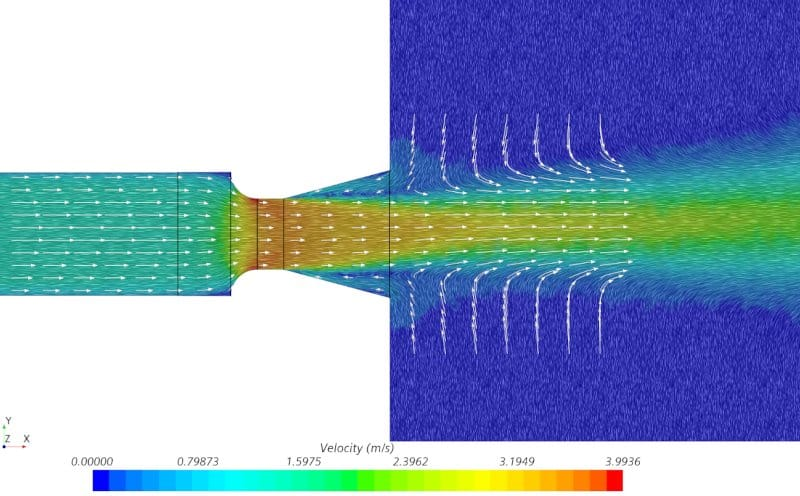
\includegraphics[width=0.7\textwidth]{flujometrias/ejemplo_lineas_corriente.jpg}
    \caption{Puerto de admisión - $10^{\circ}$@2000 RPM}\label{fig:admision_10_2000.jpg}
\end{figure}

En las tablas~\ref{tab:mapa_cd_admision} y~\ref{tab:mapa_cd_escape} se muestran los
resultados de realizar las flujometrías de los puertos de admisión y escape.

\begin{table}
  \centering
    \begin{tabular}{cccc} \toprule
      Caso  & lv        & $\Delta P$    & $C_{D}$   \\ \midrule
      0     & 0.016826  & -100331.39    &  0.213882 \\
      0     & 0.106775  & 5723.72       &  0.489375 \\
      0     & 0.016826  & -263797.72    &  0.011021 \\
      0     & 0.106775  & -3296.18      &  0.803197 \\
      0     & 0.016826  & -652902.78    &  0.011106 \\
      0     & 0.106775  & -9613.29      &  0.815804 \\
      0     & 0.016826  & -513568.73    &  0.011280 \\
      0     & 0.106775  & -3232.97      &  0.813186 \\
      1     & 0.026960  & -116996.12    &  0.375219 \\
      1     & 0.096641  & -3643.9       &  0.878414 \\
      1     & 0.026960  & -237724.11    &  0.018632 \\
      1     & 0.096641  & -6684.11      &  0.867774 \\
      1     &  0.02696  & -496509.46    &  0.111212 \\
      1     &  0.09664  & -18256.20     &  0.805830 \\
      1     & 0.026960  & -237724.11    &  0.022716 \\
      1     & 0.096641  & -6684.11      &  0.862647 \\
      2     & 0.047228  & -49343.47     &  0.541857 \\
      2     & 0.076373  & -5712.86      &  0.918061 \\
      2     & 0.047228  & -109348.67    &  0.487137 \\
      2     & 0.076373  & -17090.38     &  0.914182 \\
      3     & 0.067496  & 13.83         &  0.696967 \\
      3     & 0.071759  & -134.24       &  0.707263 \\
      3     & 0.067496  & -100073.52    &  0.731100 \\
      3     & 0.071759  & -24077.34     &  0.723965 \\
      4     & 0.075750  & -11793.31     &  0.946392 \\
      4     & 0.087764  & -33418.12     &  0.235717 \\
      4     & 0.087764  & -10715.70     &  0.221632 \\
      4     & 0.075750  & -5167.81      &  0.897169 \\
      6     & 0.123601  & -73.94        &  0.878522 \\ \bottomrule
    \end{tabular}
  \caption{Mapa de Cd del puerto de escape} \label{tab:mapa_cd_escape}
\end{table}

\begin{table}
  \centering
  \begin{tabular}{cccc} \toprule
      Caso  & lv        & $\Delta P$    & $C_{D}$   \\ \midrule
      0     & 0.014432  & -6574.97      &  0.206543 \\
      0     & 0.081937  & -87.24        &  0.828822 \\
      0     & 0.014432  & 21856.29      &  0.243975 \\
      0     & 0.081937  & -573.65       &  0.738459 \\
      0     & 0.014432  & -19738.67     &  0.222406 \\
      0     & 0.081937  & 519.60        &  0.487115 \\
      0     & 0.081937  & 1571.95       &  0.587277 \\
      0     & 0.014432  & 18077.97      &  0.256415 \\
      0     & 0.014432  & 2668.61       &  0.247292 \\
      0     & 0.081937  & 0.98          &  0.025970 \\
      2     & 0.062951  & -297.79       &  0.816487 \\
      2     & 0.081937  & 292.92        &  0.466147 \\
      2     & 0.062951  & -7374.88      &  0.980617 \\
      2     & 0.081937  & 4953.85       &  0.541619 \\
      3     & 0.071763  & 4092.13       &  0.501641 \\
      3     & 0.025832  & -3689.81      &  0.289852 \\
      4     & 0.069767  & -789.00       &  0.615690 \\
      4     & 0.069767  & 7869.92       &  0.599348 \\
      4     & 0.005564  & -12539.15     &  0.534555 \\
      4     & 0.005564  & -10091.84     &  0.583979 \\ \bottomrule
    \end{tabular}
  \caption{Mapa de Cd del puerto de Admisión} \label{tab:mapa_cd_admision}
\end{table}


La geometría obtenida luego de realizar la optimización con los mapas de Cd
incorporados a la simulación de ICESym se muestra en la figura \ref{fig:geom_nueva}.
%
Se puede ver que la geometría es similar a la inicial, siendo el puerto de
admisión algo menor en cuanto a diámetro que en el caso inicial.

Como es de esperarse, incorporar estos mapa al modelo del motor tiene un efecto
en el comportamiento del mismo, esto se puede observar principalmente en las
curvas de presión del motor.

\section{Segunda Iteración}
